\documentclass[
	12pt,
	a4paper,
	hidelinks
	]{report}
\usepackage[
	a4paper,
	left=1.9cm,
	right=1.9cm,
	top=1.9cm,
	bottom=3.17cm
	]{geometry}

\usepackage[utf8]{inputenc}
\usepackage[ngerman]{babel}
\usepackage{csquotes}
\usepackage[T1]{fontenc}

\usepackage{amsmath}
\usepackage{amsfonts}
\usepackage{amssymb}
\usepackage{graphicx}
\usepackage{pdfcomment}
\usepackage{pdfpages}

\usepackage{listings}
\usepackage{color}
\newcommand{\code}[1]{\texttt{#1}}

\usepackage{parskip}
\usepackage{setspace}
\onehalfspacing

% Akronymverzeichnis
\usepackage{hyperref}
\usepackage{array}
\usepackage{supertabular}
\usepackage{acro}
\acsetup{make-links}
\DeclareAcronym{ui}{
	short=UI,
	long = User Interface,
	sort=ui
}
\DeclareAcronym{gui}{
	short=GUI,
	long = Graphical User Interface,
	sort=gui
}
\DeclareAcronym{jre}{
	short=JRE,
	long = Java Runtime Environment,
	sort=jre
}
\DeclareAcronym{jdk}{
	short=JDK,
	long = Java Development Kit,
	sort=jdk
}
\DeclareAcronym{api}{
	short=API,
	long = Application Interface,
	sort=api
}

% Schriftarten
\usepackage{fontspec}
\setmainfont{Century Gothic}

% Kopf- und Fußzeile
\usepackage{fancyhdr}
\pagestyle{fancy}
\lhead{Team 2}
\rhead{\rightmark}
\renewcommand{\thesection}{\arabic{section}}

% Metadaten
\title{Java Banking App}
\author{Maximilian Schüller \\ Justus Siegert \\ Fynn Thierling \\ Egzon Zenuni \\ Joscha Dierks }

% Datum
\newcommand{\monthword}[1]{\ifcase#1\or Januar\or Februar\or Mär\or April\or
                                        Mai\or Juni\or Juli\or August\or
                                        September\or Oktober\or November\or Dezember\fi}
\date{\the\day. \monthword{\month} \the\year}

% Dokument
\begin{document}
\maketitle
\tableofcontents
\newpage

\section{Einleitung}
Das Projekt >> Java Banking App << ist eine Java Anwendung mit einer Datenbankschnittstelle und einem \ac{ui}, genauer ein \ac{gui}. Ziel ist es, eine intuitiv bedienbare Anwendung zu schaffen, die die vorgegebenen Funktionsparameter erfüllt.

\section{Anforderungen an das Projekt}
Das Projekt sollte ein \ac{ui} umgesetzt mit der Technologie von \code{Java Swing} besitzen. Alternativ stand \code{Java AWT} zur Auswahl, jedoch haben wir dies nicht direkt genutzt. Zu erwähnen ist jedoch, dass \code{Java Swing} ein Nachfolger von \code{Java AWT} ist und darauf basiert, jedoch weitaus mehr Funktionen bietet. Außerdem ist \code{Java Swing} deutlich performanceschonender und unterstützt das native Design der einzelenen Betriebssysteme, ohne dass dafür eine direkte Spezifikation erforderlich ist. Dies macht die plattformunabhängige Programmierung deutlich einfacher.

Weiterhin ist es erforderlich, dass das Programm seine Daten dauerhaft speichert, also auch bei einem Neustart die Daten aus der letzten Sitzung wieder geladen werden.

Ein realistisches Klassenmodell mit sinnvoll verteilten Attributen und Methoden, einer Vererbunghierarchie, und abstrakten Klassen muss ebenso vorhanden sein. Eventuell wird hierbei auf Polymorphie und Datenkapselung gesetzt.

Eine durchgehende und nutzerfreundliche Fehlerbehandlung wird vorausgesetzt, besonders Nutzereingaben, Konvertierungen und Überläufe sind hierbei zu berücksichtigen.

Der Programmcode folgt keinen explizieten Vorgaben, jedoch wird auf eine konsistente Formatierung und sinnvolle Bezeichnungen geachtet.

\newpage

\section{Projektplanung}
Die vorausgehende Projektplanung ist spartanisch ausgefallen, um schnellstmöglich das Produkt fertig zu stellen. Daher beschränkt sich diese auf einen groben Aufbau des \ac{gui} und die nötigen Funktionsweisen. Wir einigten uns darauf, uns auf ein Hauptfenster zu beschränken, dass entweder die Transaktionsübersicht oder das Administrator-Dashboard anzeigt. Darüber hinaus sollen alle Funktionen ein eigenes Popup Fenster erhalten.

Der Zeitplan beinhaltet das Ziel, alle Module und Funktionen bis zum 23. Juni 2023 fertigzustellen, um die darauffolgenden Tage die Zusammenführung derselben und das finale Debuggen vornehmen zu können.

\subsection{Klassenmodell}
\begin{figure}[!h]
	\makebox[\textwidth][c]{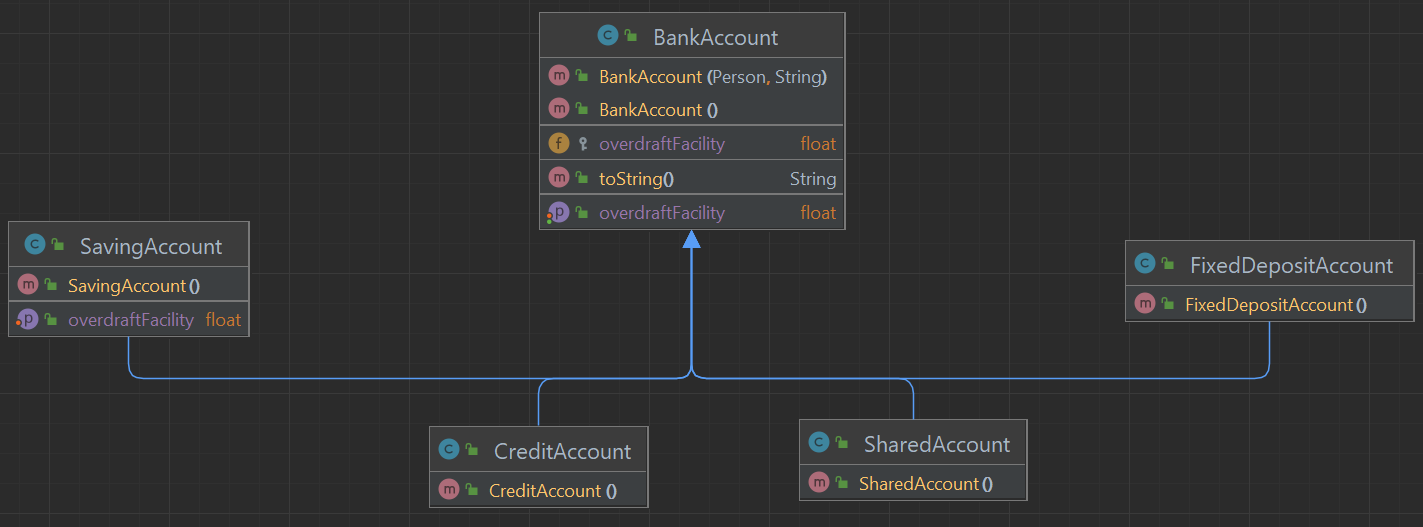
\includegraphics[width=\textwidth]{importent_classes.png}}
\end{figure}
Das Klassenmodell leitet die verschiedenen Bankkonten von einem Standartkonto ab. Die Unterklassen ergänzen die Felder des Standartkontos. Die Funktionalität des Standartkontos wird durch die abgeleiteten Klassen tweilweise erweitert oder verändert. Ein Beispiel hierfür ist, dass ein Sparkonto die Funktion \code{setOverdraftFacility()} überschreibt, da ein Sparkonto nicht überzogen werden darf.

Die beiliegende vollständige Projektdokumentation, die mithilfe des Tools \code{Javadoc} erstellt wurde, liefert nähere Informationen über die einzelenen Felder und Methoden. Auf der folgenden Seite ist das Vollständige Klassendiagramm des Projekts zu sehen.

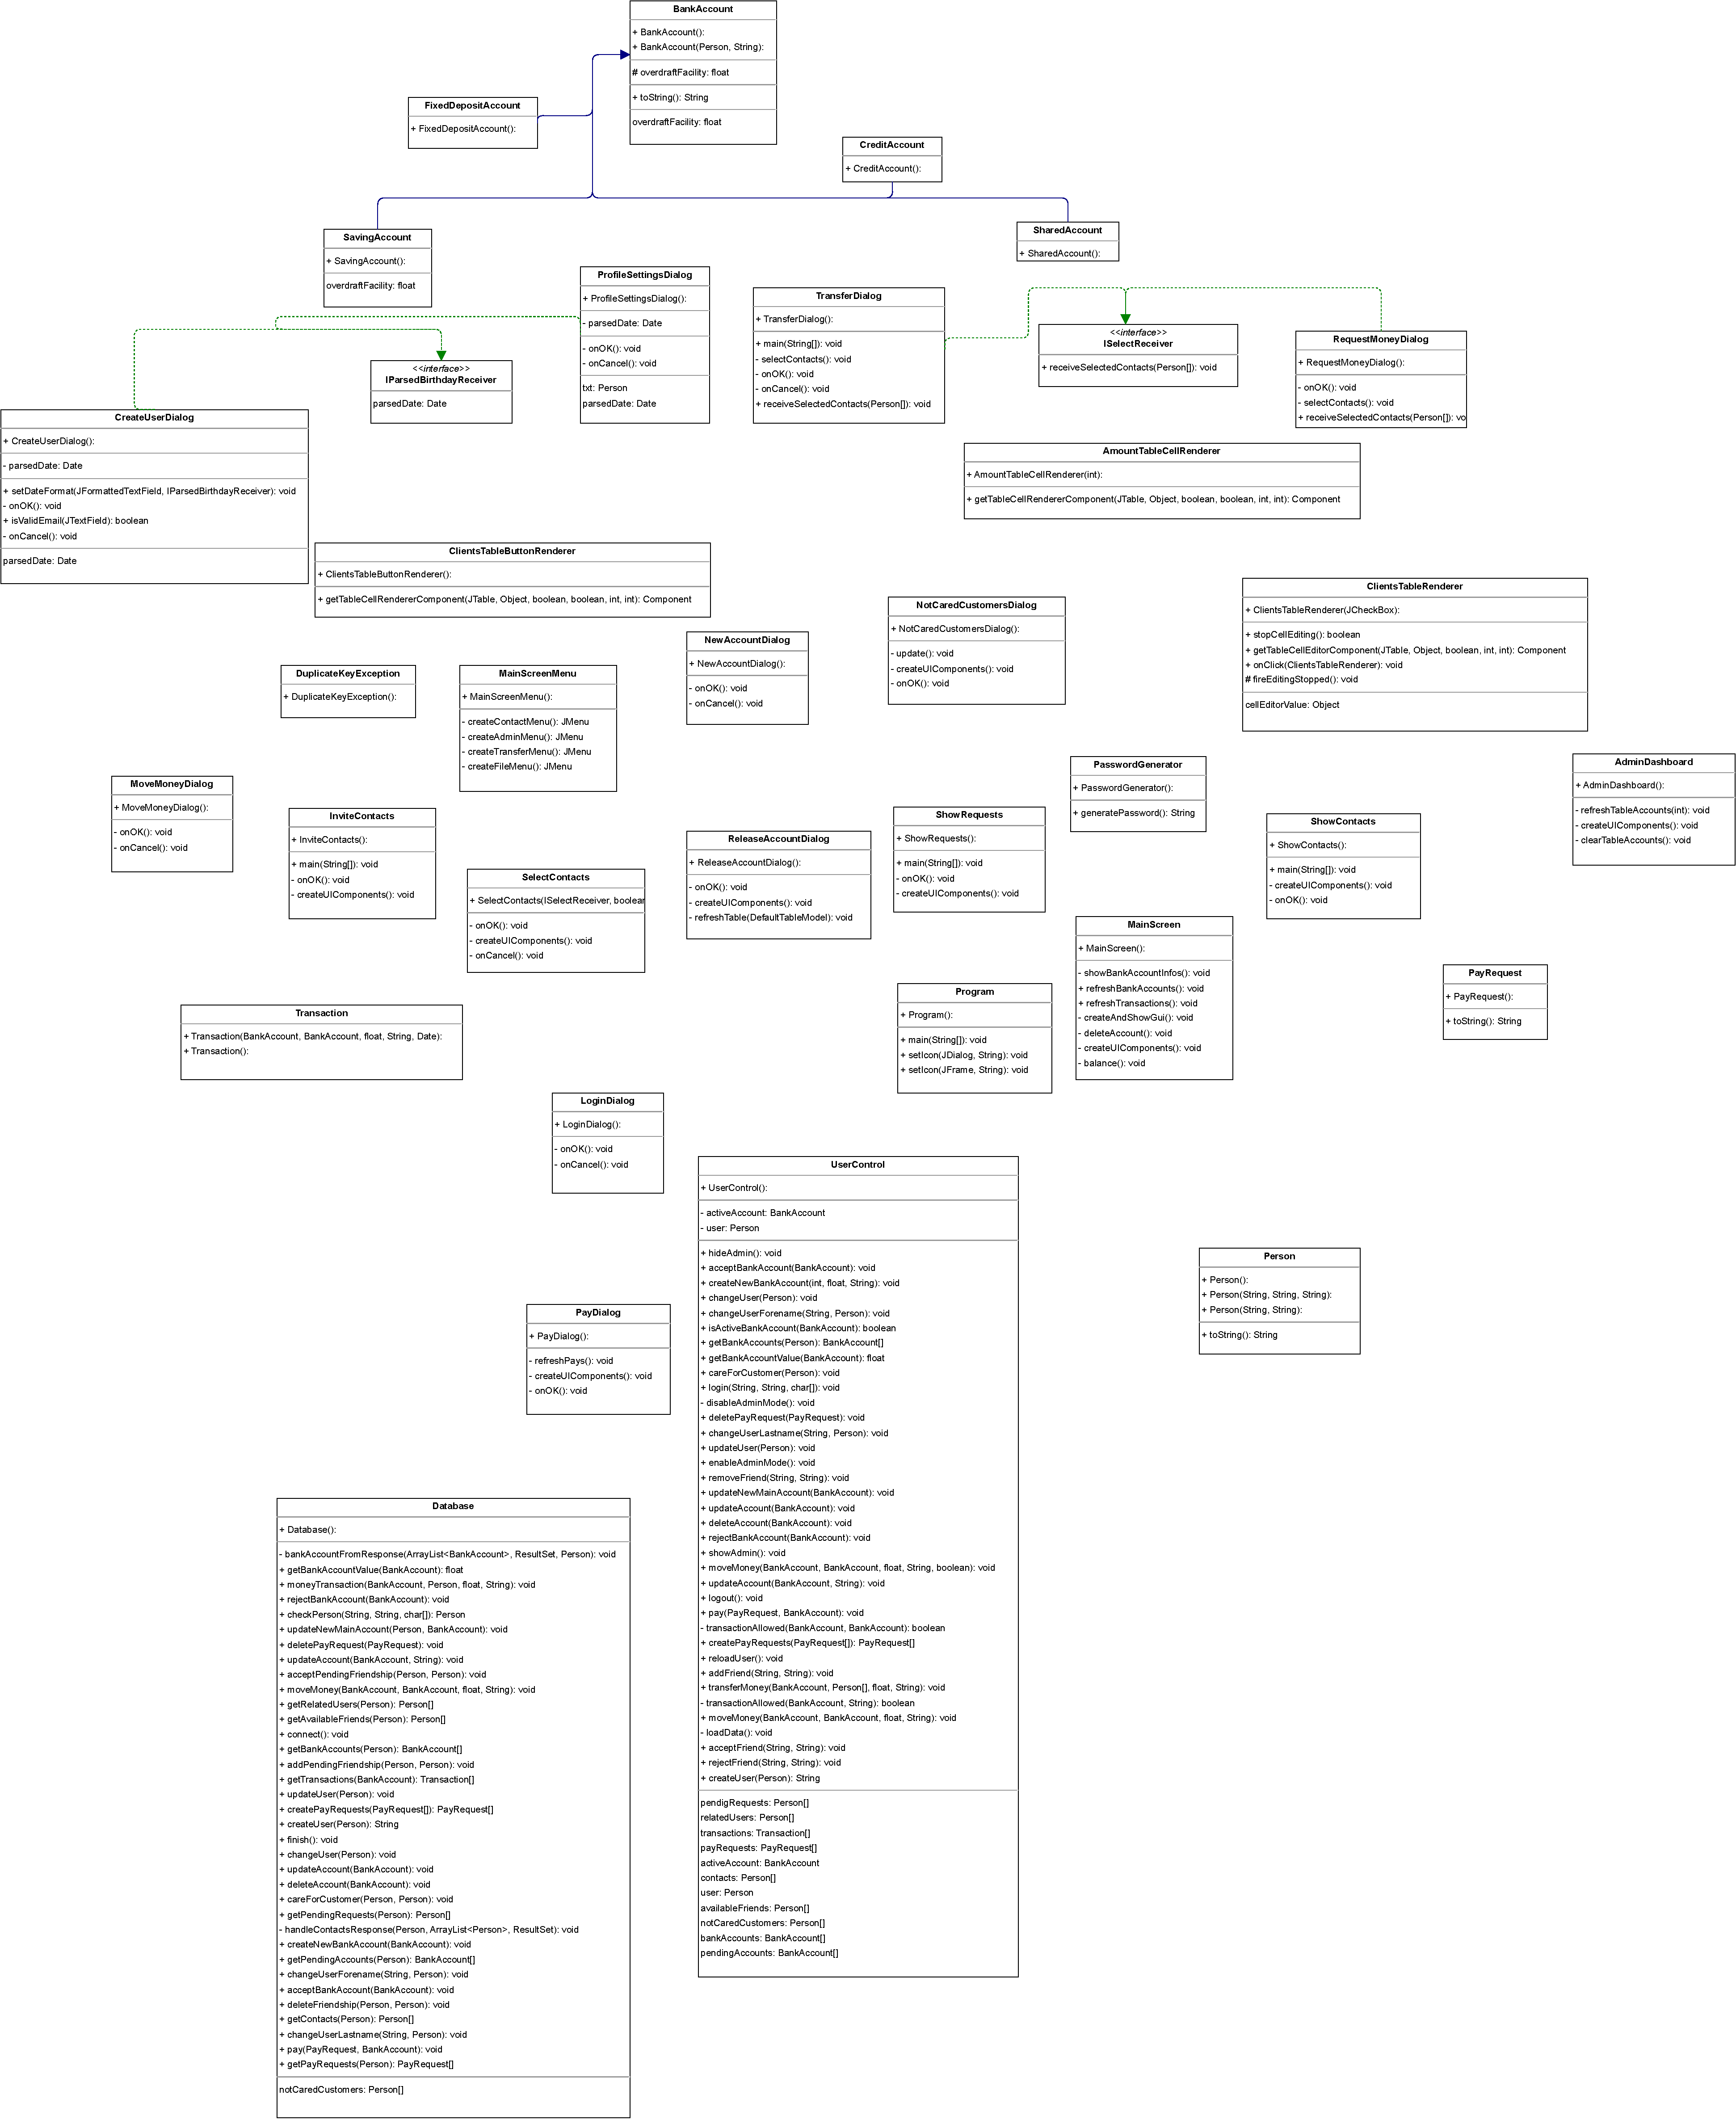
\includepdf[pages=-]{class_diagramm.pdf}

\section{Installationsanleitung}
Zum ausführen des Programms kann das beiliegende \code{jav} Archiv über die Konsole gestartet werden. Dazu wird der Befehl \code{\$ java -jar Banking.jar} im Verzeichnis ausgeführt, welches das Archiv enthält.

Voraussetzung, um diesen Befehl ausführen zu können, ist die vollständige Installation des \ac{jre} der Version 19 oder höher. Sollte das \ac{jdk} bereits vorhanden sein, kann auch dieses genutzt werden, um das JAR-Archiv auszuführen. Hier kann das \ac{jre} heruntergeladen werden \url{https://www.oracle.com/java/technologies/downloads/#jdk20-windows}. Es sollte sichergestellt werden, dass der Ordner \code{bin} im Installationsverzeichnis des \ac{jre} den Umgebungsvariabeln hinzugefügt wurde, bevor der Befehl in der Konsole ausgeführt wird.

Damit die Anwendung korrekt funktioniert, ist eine aktive Internetverbindung erforderlich!

\section{Externe Software}
Das Programm verwendet eine externe zentrale Datenbank, sodass jeder Client von überall auf der Welt mit einer Internetverbindung auf unseren Service zugreifen kann. Unser Applikation greift direkt vom Client auf die Datenbank zu. Dies ist in einer produktiven Umgebung \textbf{nicht} zu empfehlen! Die Zugangsdaten zur Datenbank stehen im Code des Clients und können mit verhältnismäßig wenig Aufwand ausgelesen werden. Ein Angreifer kann sich so leicht Zugriff zu Datenbank verschaffen.

Zu empfehlen ist es, ein \ac{api} zwischen Client und Datenbank zu stellen, der die Authentifizierung der Nutzer übernimmt. So wird verhindert, dass ein Nutzer direkt auf die Datenbank zugreifen kann, er erhält also nur seine Anmeldedaten für sein Konto, aber niemals die Anmeldedaten für weiter Infrastrucktur.

Wir haben uns gegen dieses bewährte Modell entschieden, da der Arbeitsaufwand sich effektiv verdoppelt hätte, hätten wir ein \ac{api} zu unserer Anwendung geschrieben. Da unsere Applikation nicht produktiv eingesetzt wird, sondern nur ausgewählten Personen zur Verfügung steht, ist das Risiko akzeptabel. Uns ist jedoch bewusst, dass in einer produktiven Umgebung ein solches Modell extrem unsicher ist.
\newpage
\subsection{Datenbank}
Als Datenbank verwenden wir eine MariaDB \code{Ver 15.1 Distrib 10.6.12-MariaDB} auf einem \code{Ubuntu 22.04.2 LTS} V-Server.

Zum Verbinden mit der Datenbank verwenden wir die externe Bibliothek \\
 \code{org.mariadb.jdbc.Driver} der Version \code{3.1.4}, die hier heruntergeladen werden kann: \url{https://mariadb.com/downloads/connectors/connectors-data-access/java8-connector}
 \begin{figure}[!h]
	\makebox[\textwidth][c]{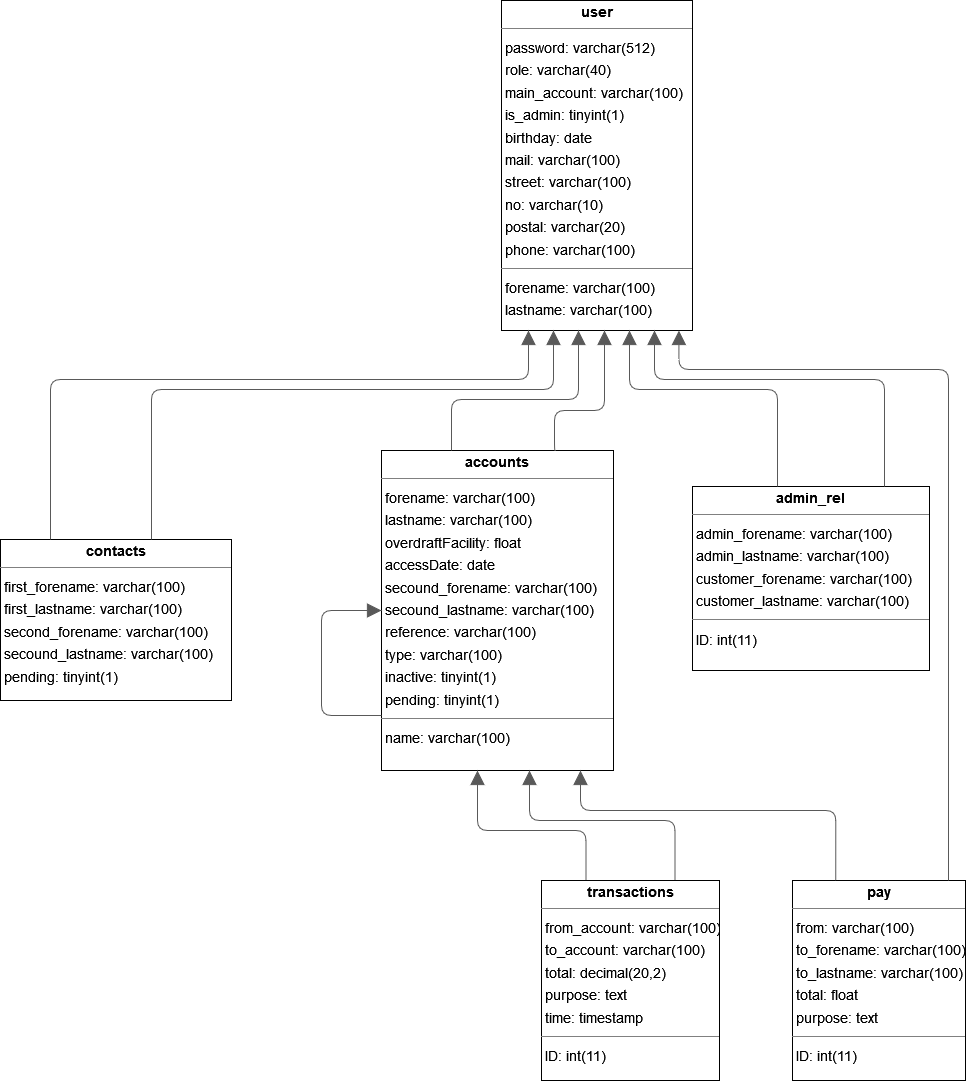
\includegraphics[width=\textwidth]{database_rel_diagram.png}}
\end{figure}


\newpage
\phantomsection
	\addcontentsline{toc}{chapter}{Abkürzungen}
	\printacronyms[template=supertabular]

\end{document}